% !TEX encoding = UTF-8 Unicode

% Beispiel für ein LaTeX-Dokument im Format "seminarvorlage"
\documentclass[ngerman]{seminarbeitrag}
% ngerman = Deutsch in neuer Rechtschreibung
% english = Englisch

\usepackage[utf8]{inputenc} % Kodierung der Non-ASCII-Zeichen
\usepackage{listings} %Einfügen von Code-Beispielen
\usepackage{xcolor}
\usepackage{subfig}
\usepackage{float}

\begin{document}

%Einstellungen für Listings
\lstset{basicstyle=\small\ttfamily, language=C, keywordstyle=\color{black},commentstyle=\color{gray}, numbers=left, numberstyle=\tiny,emph={Function, if, then, else, End, while, for, each},emphstyle=\bfseries, breaklines=true, breakatwhitespace=True, captionpos=b, escapeinside={(*}{*)}}
% Unbedingt notwendig: Titel, Autoren
\title{Gleichmäßige Flächenaufteilung von Polygonen}
\author{Sebastian Loder\and\ Jan Steffen Jendrny}

\maketitle% Titelangaben produzieren, kein Inhaltsverzeichnis

\begin{abstract}
In dieser Arbeit wird ein konkretes Problem der Polygonzerlegung, das sogenannte \emph{Problem der verankerten Flächenaufteilung} (eng. \emph{anchored area partition problem}) vorgestellt, welches von Susan Hert und Vladimir Lumelsky \cite{Hert.1998} veröffentlicht wurde. Die vorliegende Arbeit basiert maßgebend auf dieser Veröffentlichung und beschreibt, wie dieses Problem mittels \emph{sweepline-} und \emph{divide-and-conquer}-Techniken effizient gelöst werden kann. Die Lösung erfolgt zunächst für konvexe Polygone und wird anschließend auf nicht konvexe, nicht einfache Polygone erweitert.

\keywords{Polygonzerlegung, Flächenaufteilung, Flächenerkundung, Roboterplanung}% Keywords innerhalb vom Abstract
\end{abstract}

% Section-Überschriften werden automatisch in GROSSBUCHSTABEN gesetzt
\section{Einleitung}\label{einleitung}
Die Polygonzerlegung ist eines der zentralen Probleme in der algorithmischen Geometrie und hat viele Anwendungsfälle, wie beispielsweise in der Kartographie,
Bildverarbeitung oder in der Computergrafik. In vielen Fällen wird die Polygonzerlegung benötigt, um aus einem beliebigen Polygon eine Menge von Teilpolygonen mit bestimmten
Eigenschaften zu berechnen. Als Beispiel einer vielfach verwendeten Polygonzerlegung kann die Triangulation genannt werden, bei welcher ein gegebenes Polygon in eine Menge von Dreiecken
zerlegt wird. Für die so berechnete Menge von Dreiecken stehen dann effiziente Algorithmen zur Lösung von Problemen zur Verfügung. Anschließend können die Lösungen der Teilpolygone zu
einer Lösung für das Ausgangspolygon zusammengefasst werden. \\

Bei dem hier vorgestellten Problem der verankerten Flächenaufteilung ist die Anforderung an die resultierenden Teilpolygone nicht durch eine bestimmte Geometrie
(z. B. ein Dreieck), sondern durch die Lage und Fläche der Teilpolygone gegeben. Bezüglich der Lage besteht die Anforderung darin, dass ein gegebener Punkt (Standort genannt) auf
dem resultierenden Polygon liegen muss. Jeder Standort weist als Eigenschaft eine Flächenanforderung auf, welche durch die Größe des Teilpolygons erfüllt werden soll. Die
Flächenanforderung kann je Standort den gleichen Wert aufweisen, kann aber auch unter den Standorten variieren. Somit bezieht sich das hier beschriebene Problem sowohl auf eine
gleichmäßige, als auch eine ungleichmäßige Flächenaufteilung. Das beschriebene Problem ist unter anderem durch die Flächenerkundung von Robotern motiviert: \\

Auf einem Polygon werden n Roboter auf Standorten $S_{i},$ \iton positioniert, welche die Aufgabe erhalten, zusammen die gesamte Fläche des Polygons zu
erkunden. Hierzu muss jede Position innerhalb des Polygons von einem der n Roboter abgefahren werden. Um die Arbeit unter den Robotern aufzuteilen, ist es sinnvoll, jedem Roboter einen Polygonteil zuzuweisen, der jeweils zu bearbeiten ist. Die Teilpolygone sollen sich nicht überlappen, um ein mehrfaches Überfahren zu vermeiden. Bei der Flächenaufteilung muss berücksichtigt werden, dass der Startpunkt eines jeden Roboters auf dem zugewiesenen Teilpolygon beziehungsweise in diesem liegt. Eine unterschiedliche Leistung der Roboter kann über die Flächenanforderung je Standort berücksichtigt werden. \\

Zur formalen Beschreibung des Problems sind als Eingangsdaten ein Polygon $P$ sowie eine (nicht leere) Liste von Standorten $S(P)$ gegeben. Für jeden der $n$
Standorte \si, \iton ist der benötigte Flächenanteil $c_{i}$, \iton mit $0 < c_{i} < 1$ gegeben, sodass $\sum_{i=1}^{n}c_{i}=1.0$ gilt. Das Polygon $P$ soll in $n$, nicht
überlappende Polygone zerlegt werden, sodass jeder Standort \si auf dem Teilpolygon \pi mit Fläche $c_{i}* \mar{P}$ liegt. Aus der Fläche des Polygons $P$ kann für jeden der $n$ Standorte die benötigte Fläche mit $c_{i}* \mar{P}$ bestimmt werden.\\

In der Praxis werden Flächenaufteilungen beispielsweise bei der Einteilung von Zustellbezirken der Post oder Einsatzgebieten von Rettungskräften verwendet. Die zuvor beschriebene, konkrete Problembeschreibung der verankerten Flächenaufteilung kann in Bezug auf die Roboterplanung beispielsweise auf Saug- oder Mähroboter übertragen werden, welche inzwischen in einigen Haushalten zu finden sind.\\

Hinweis: Die in dieser Arbeiten genutzten Begriffe und Abkürzungen sind aus der Veröffentlichung von Hert und Lumelsky \cite{Hert.1998} übernommen und werden in Kapitel~\ref{begriffe} erläutert. Die Listings wurden gegenüber der Veröffentlichung \cite{Hert.1998} zur besseren Lesbarkeit verändert.



% Aufteilung eines Polygons im konvexen Fall
\section{Aufteilung eines einfachen, konvexen Polygons}\label{konvex}
%Beschreibung der Grundidee
\subsection{Grundidee}\label{grundidee konvex}
Bei der nachfolgend beschriebenen Lösung des Problems wird ein konvexes Eingabepolygon \cp mithilfe von Liniensegmenten schrittweise zerlegt. Jedes Liniensegment
\l ist hierbei vom Startpunkt \ls zum Endpunkt \Le orientiert, wobei beide Punkte auf dem Rand von \cp liegen. Wenn für \ls und \Le eine Position gefunden wurde, erfolgt eine Zerlegung in zwei Teilpolygone.
Die bei jeder Teilung entstehende Teilpolygone erhalten entsprechend ihrer Lage zum Liniensegment \l die Bezeichnungen \prl für das rechts und \pll für das links
des Liniensegments liegenden Polygons, wobei angenommen wird, dass hierbei die Blickrichtung von \ls nach \Le orientiert ist. Die Liniensegmente (bzw. \ls und $L_{e}$) werden so positioniert, dass die Fläche von \prl der benötigten Fläche der auf dem Rand von \prl liegenden Standorte entspricht (\pll analog). Die Zerlegung wird für jedes Teilpolygon \prl und \pll rekursiv aufgerufen, bis nur noch 1-Standort Polygone vorliegen. Hierbei sei betont, dass aus einer Zerlegung eines konvexen Polygons durch ein Liniensegment immer zwei konvexe Polygone und insbesondere kein nicht konvexes Polygon resultiert.

% Beschreibung des vorgestellten Algorithmus
\subsection{Aufteilung eines einfachen, konvexen Polygons}\label{aufteilung konvex}
Aus \cp entstehende, konvexe Polygone werden mit \cpi notiert. Mit den genannten Überlegungen lässt sich ein rekursiver \emph{divide-and-conquer} - Algorithmus
zur Flächenaufteilung eines konvexen Polygons - basierend auf n Standorten - wie in Listing~\ref{code grundidee} skizzieren.

\begin{lstlisting}[float,caption={Die Grundidee hinter dem Algorithmus \con}, frame=single, label=code grundidee]
// Input: Convex polygon CP
Function ConvexDivide(CP)
    if Length(S(CP)) == 1 then return CP
    // Here, the postion of L has to be calculated
    PrL, PlL = Cut(CP, L)   // CP is cut into two pieces PrL and PlL
    ConvexDivide(PrL)   // recursive PrL
    ConvexDivide(PlL)   // recursive PlL
 End ConvexDivide() 
\end{lstlisting}

Bei jedem Aufruf von \textit{ConvexDivide}($CP$) wird zunächst geprüft, ob das übergebene Polygon nur noch einen Standort enthält. Falls ja, ist der Zielzustand für dasübergebene Polygon erreicht und es ist keine weitere Flächenaufteilung erforderlich. Falls das Polygon mehrere Standorte enthält, erfolgt eine weitere Aufteilung
des Polygons in zwei Teilpolygone \prl und $\mpll$, welche dann rekursiv mit \con aufgerufen werden.\\

\begin{figure}[ht]
    \subfloat[]{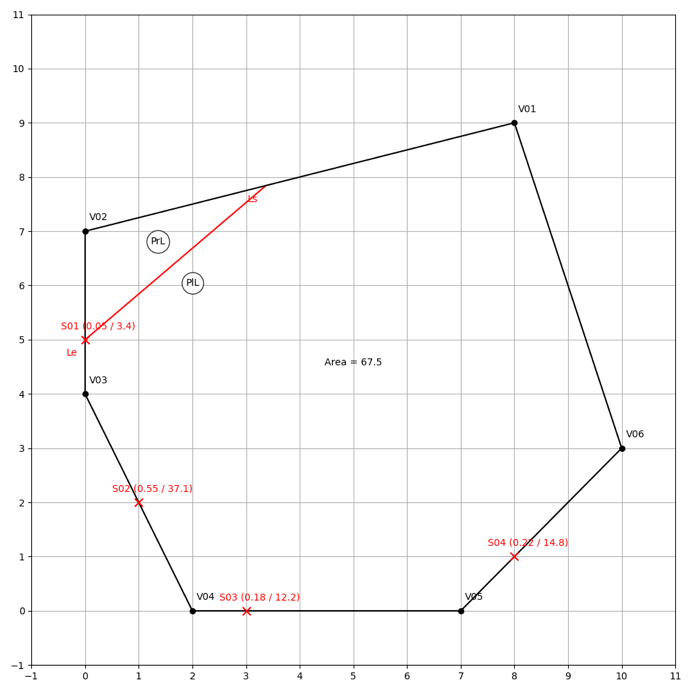
\includegraphics[width=0.25\textwidth]{./Abbildungen/1a.png}}
    \subfloat[]{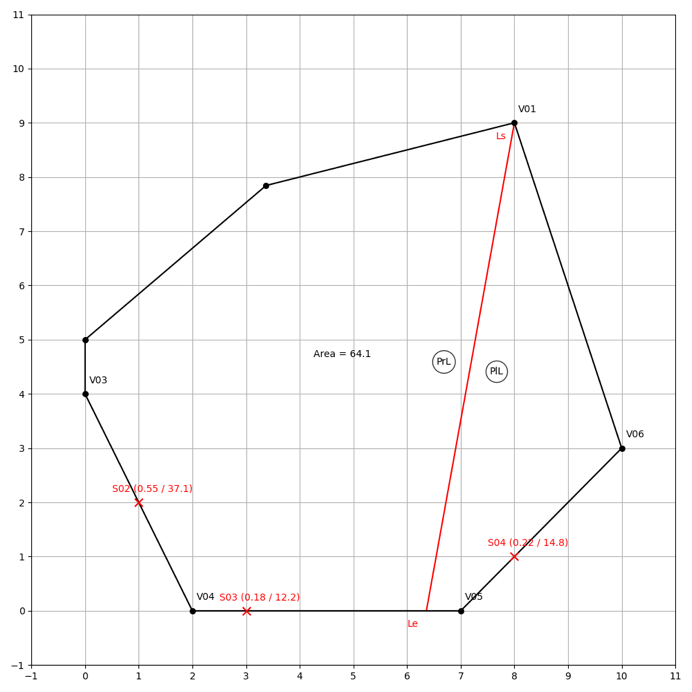
\includegraphics[width=0.25\textwidth]{./Abbildungen/1b.png}}
    \subfloat[]{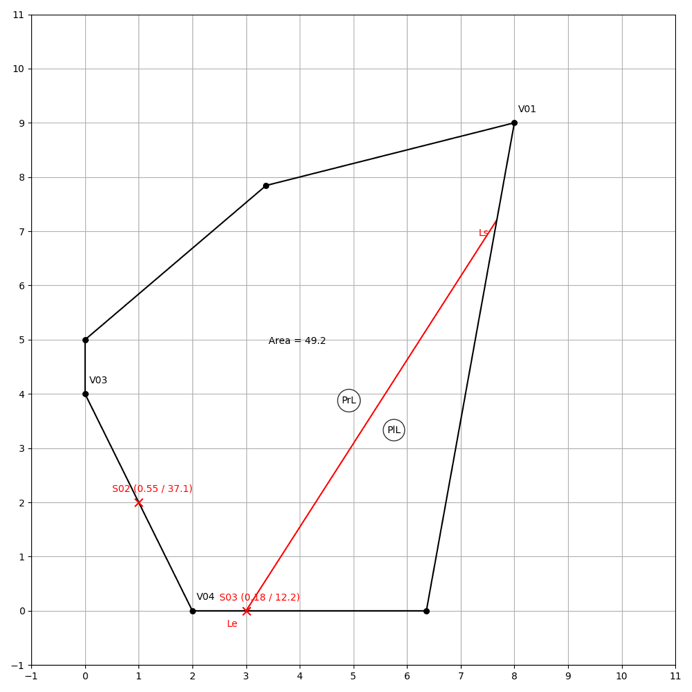
\includegraphics[width=0.25\textwidth]{./Abbildungen/1c.png}}
    \subfloat[]{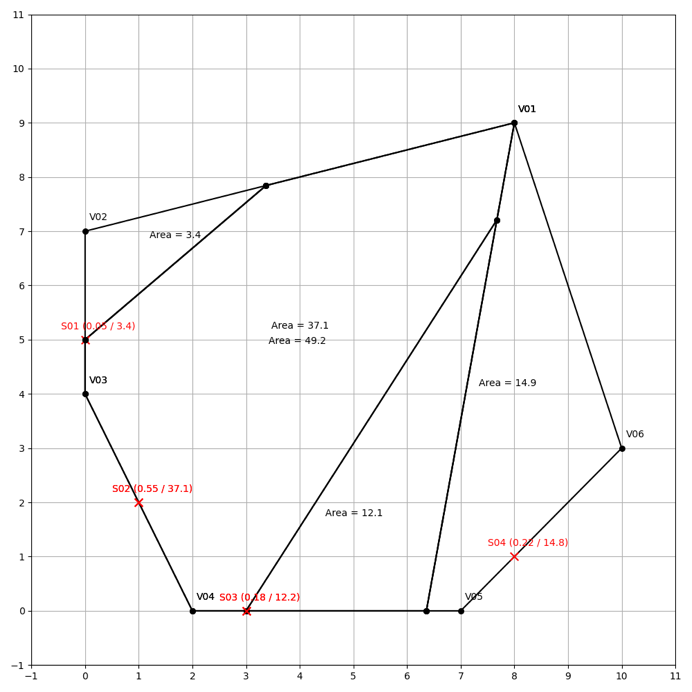
\includegraphics[width=0.25\textwidth]{./Abbildungen/1d.png}}
    \centering
    \caption{Zerlegung eines konvexen Polygons $CP$ in vier konvexe Polygone $CP_{1},...,CP_{4}$}
    \label{erstes beispiel}
\end{figure}

Abbildung~\ref{erstes beispiel} zeigt ein Beispiel für eine Zerlegung eines 4-Standort-Polygons in 4 Teilpolygone mit jeweils einem Standort. In (a) wird \prl mit einer Fläche von 3.4 FE abgetrennt und dem Standort $S01$ zugeordnet. Die in (b) entstehenden Teilpolygone \prl und \pll weisen eine Fläche von 49.3 FE beziehungsweise 14.8 FE auf. Letzteres wird dem Standort $S04$ zugeordnet und ist als 1-Standort-Polygon fertig bearbeitet. \prl wird in (c) erneut aufgeteilt, sodass die Flächenanforderung von $S02$ und $S03$ jeweils erfüllt werden. (d) zeigt die resultierende Aufteilung mit 4 Teilpolygonen.  


%Beschreibung, wie die Linie L das Polygon durchläuft
\subsection{Positionierung der Schnittlinie}\label{schnittlinie konvex}

Aus vorangegangenem Kapitel bleibt offen, wie genau die Aufteilung eines konvexen Polygons \cp in die Polygone \prl und \pll erfolgt, sodass anschließend
$\mar{\mprl}=\marreq{S_{1},...,S_{i}}$ und $\mar{\mpll}=\marreq{S_{i+1},...,S_{n}} $ gilt.
Konkret ist zu klären, wie Anfangs- und Endpunkt der Schnittlinien positioniert werden (siehe Listing~\ref{code grundidee}, Zeile 4). Zunächst werden \ls und \Le beim Aufruf von \con wie folgt initialisiert:

\begin{itemize}
\item Der Startpunkt \ls der Linie \l wird mit den Koordinaten des ersten Punkts der Liste \w initialisiert, wobei dieser nach Definition ein Polygonpunkt (und
kein Standort) ist. Es gilt daher $w_{1} \in V()$.
\item Der Endpunkt \Le wird mit den Koordinaten des ersten Standorts in \w initialisiert und mit $w_{k}$ notiert, wobei $k$ der Index in \w ist, bei dem der
erste Standort liegt. Da die Standorte nach ihrem Vorkommen auf dem Weg von $v_{1}$ nach $v_{l}$ geordnet sind, ist bei einem konvexen Polygon sichergestellt,
dass die Standorte $S_{2},…,S_{n}$ alle links der Linie L liegen.
\end{itemize}

Bei einer Zerlegung mit einer so initialisierten Linie würde $S(\mprl)=S_{1}$ und $S(\mpll)=S_{2},...,S_{n}$ gelten, wobei $S_{1}$ in einer Ecke von \prl
liegen würde. Je nach Fläche von \prl und \arreq{S_{1}} werden folgende Fälle unterschieden: \\

\textbf{Fall 1: $\mar{\mprl}>\marreq{S_{1}}$} \\
Nach der Initialisierung der Linie \l wird festgestellt, dass die Fläche von \prl größer ist als die benötigte Fläche von $S_{1}$. In diesem Fall erfolgt eine
Verkleinerung von \ar{\mprl} unter Beibehaltung von $S(\mprl)=S_{1}$. Dies geschieht, indem \Le als Drehpunkt fungiert und \ls inkrementell gegen den Uhrzeigersinn entlang des Polygons
verschoben wird, bis $\mar{\mprl}=\marreq{S_{1}}$ gilt. Zur Verdeutlichung dieser Vorgehensweise sollen folgende Punkte nochmals herausgestellt werden:

\begin{itemize}
\item Durch die Initialisierung kann auf dem Weg von $w_{1}$ zu $w_{k}$ kein weiterer Standort liegen, d.h. $\marreq{S(\mprl)}$ ist konstant.
\item $\mar{\mprl}$ wird mit Verschiebung von \ls stetig kleiner. Bei $L_{s}=S_{1}$ gilt $\mar{\mprl}=0$.
\item \Le ist fest, d.h. \s{1}ist stets Teil von $\mprl$.
\end{itemize}

Wenn die Bedingung $\mar{\mprl}=\marreq{S_{1}}$ eintritt, erfolgt eine Polygonzerlegung. Für \prl erfolgt keine weitere Zerlegung beim Aufruf von
\con (siehe Listing~\ref{code grundidee}, Zeile 3), da nur $S_{1}$ auf dessen Rand liegt. Falls auf dem Rand von \pll mehr als ein Standort verbleibt, erfolgt eine erneute
Zerlegung beim Aufruf von \con($\mpll$) (siehe Listing~\ref{code grundidee}, Zeile 7).\\

\textbf{Fall 2: $\mar{\mprl}<\marreq{S_{1}}$} \\
Nach der Initialisierung der Linie \l wird festgestellt, dass die Fläche von \prl kleiner ist als die benötigte Fläche von $S_{1}$. In diesem Fall erfolgt eine Vergrößerung von \ar{\mprl}mit dem Ziel, die Flächenanforderung zu erfüllen. Hierbei fungiert \ls als Drehpunkt und \Le wird auf den nächsten in \w vorkommenden Polygonpunkt oder Standort $w_{k+1}$ gesetzt. Die Anforderung wird erneut geprüft. In diesem Schritt wird \Le von Polygonpunkt zu Polygonpunkt verschoben. Eine inkrementelle Verschiebung entlang des Polygons erfolgt dann unter Fall 2.1 beziehungsweise 2.2.

Hierbei kann es nun vorkommen, dass \Le auf die Koordinaten eines Punktes $w_{j}$ in \w gesetzt wird, welcher ein Standort $\ne S_{1}$ ist. Dieser Standort wird dann beim nächsten Vorrücken (also bei $w_{j+1}$) zur benötigten Fläche von \prl hinzugenommen. Bei Fall 2 kann \arreq{\mprl} demnach ansteigen, sodass ein Vorücken von \Le zwar zu einer größeren Fläche von $\mprl$, nicht aber unbedingt zu einem günstigeren Verhältnis aus $\mar{\mprl} / \marreq{S(\mprl)}$ führt. \\
\Le wird so oft verschoben, bis eine der folgenden Bedingungen eintritt:\\

\begin{itemize}
\item $\mar{\mprl}>\marreq{S(\mprl)}$
\item $L_{e} = S_{n}$
\end{itemize}

Je nachdem, wie weit \Le vorrückt und wie groß die Fläche von \prl im Vergleich zur Flächenanforderung von S($\mprl$) ist, werden nun weiter zwei Fälle unterschieden:\\

\textbf{Fall 2.1: $L_{e} = S_{n}$ und $\mar{\mprl}>\marreq{S(\mprl)}$} \\
In diesem Fall wird der Endpunkt \Le inkrementell im Uhrzeigersinn entlang des Polygons bewegt, bis $\mar{\mprl}=\marreq{S(\mprl)}$ gilt.
Hinweis: Angenommen die Ausgangsposition von \Le ist $w_{j}$, dann muss es zwischen $w_{j}$ und $w_{j-1}$ eine Position geben, bei der $\mar{\mprl}=\marreq{S(\mprl)}$ gilt, da beim Vorrücken \ar{\mprl} bei $w_{j-1}$ zu klein und bei $w_{j}$ zu groß war. Dieser Zwischenpunkt wird durch Interpolation gefunden.\\

\textbf{Fall 2.2: $L_{e} = S_{n}$ und $\mar{\mprl}<\marreq{S(\mprl)}$} \\
In diesem Fall wird der Anfangspunkt \ls inkrementell im Uhrzeigersinn entlang des Polygons bewegt, bis $\mar{\mprl}=\marreq{S(\mprl)}$ gilt.

Diese Vorgehensweise entspricht im Wesentlichen Fall 1, wobei \ls (initialisiert mit $w_{1}$) nun nicht gegen den Uhrzeigersinn zum ersten Standort $S_{1}$, sondern im Uhrzeigersinn zum letzten Standort \s{n}bewegt wird. Vergleiche auch Abbildung~\ref{zweites beispiel}, Fall (c) und (i).\\

\begin{figure}[hb]
    \subfloat[]{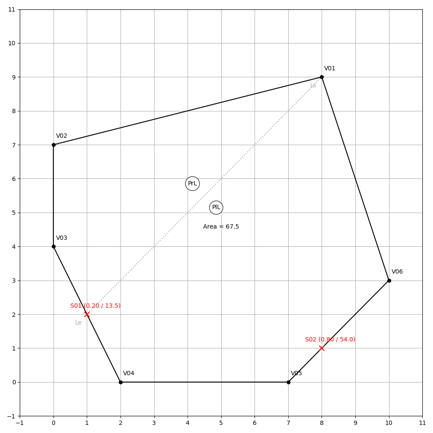
\includegraphics[width=0.30\textwidth]{./Abbildungen/2a.png}}
    \subfloat[]{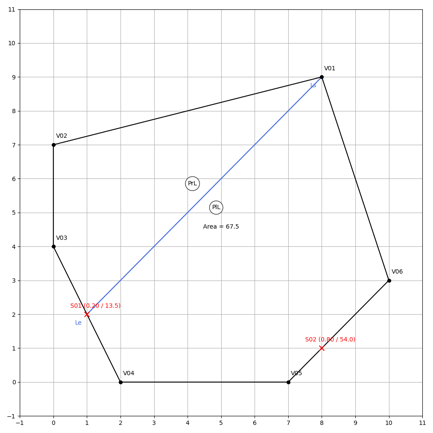
\includegraphics[width=0.30\textwidth]{./Abbildungen/2b.png}}
    \subfloat[]{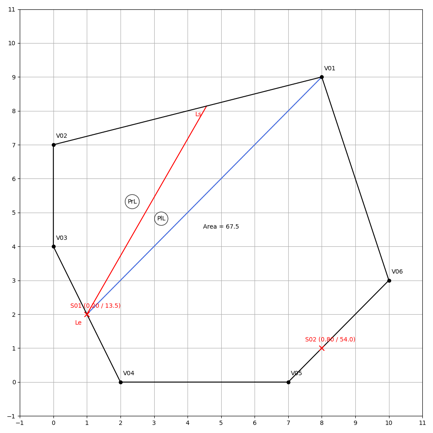
\includegraphics[width=0.30\textwidth]{./Abbildungen/2c.png}}
    \qquad
    \subfloat[]{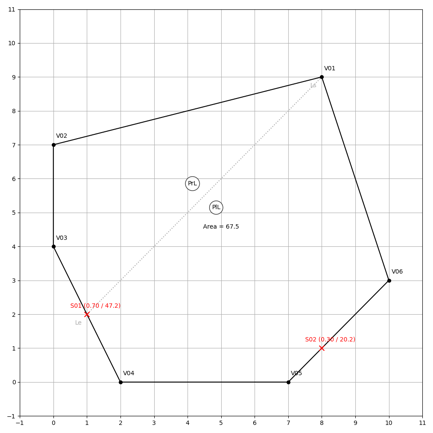
\includegraphics[width=0.30\textwidth]{./Abbildungen/2d.png}}
    \subfloat[]{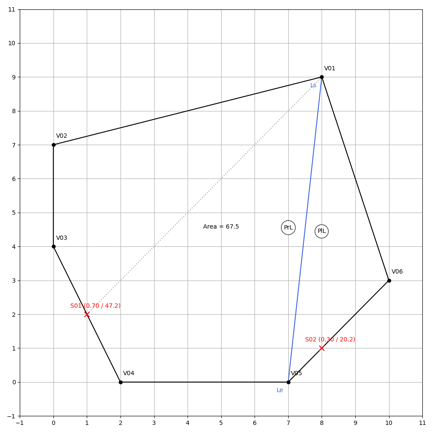
\includegraphics[width=0.30\textwidth]{./Abbildungen/2e.png}}
    \subfloat[]{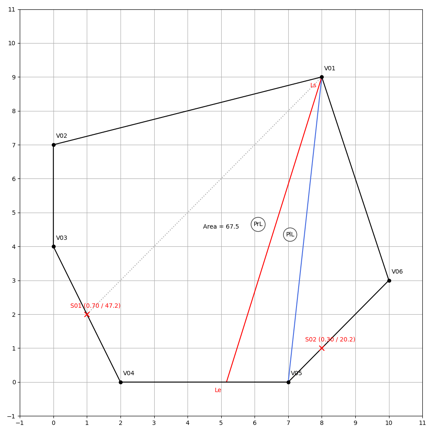
\includegraphics[width=0.30\textwidth]{./Abbildungen/2f.png}}
    \qquad
    \subfloat[]{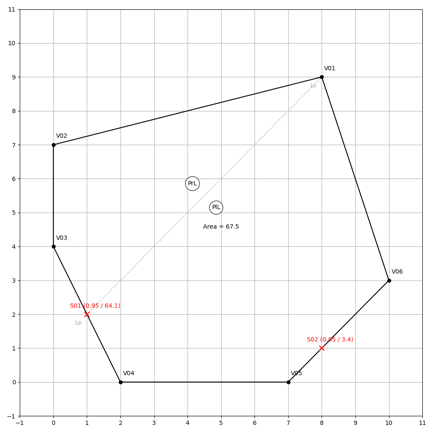
\includegraphics[width=0.30\textwidth]{./Abbildungen/2g.png}}
    \subfloat[]{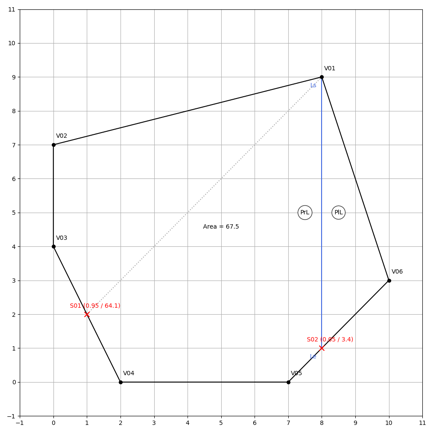
\includegraphics[width=0.30\textwidth]{./Abbildungen/2h.png}}
    \subfloat[]{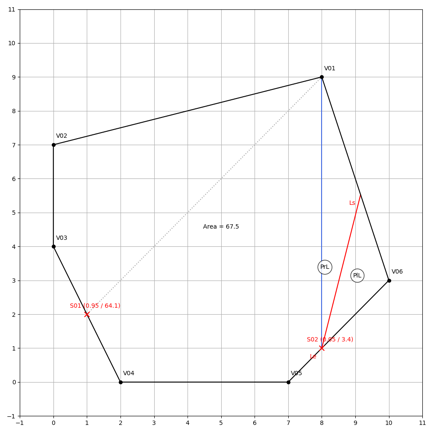
\includegraphics[width=0.30\textwidth]{./Abbildungen/2i.png}}
    \centering
    \caption{Fall 1, 2.1 und 2.2 inklusive der jeweiligen Zwischenschritte im Algorithmus \mbox{\textit{ConvexDivide}}.}
    \label{zweites beispiel}
\end{figure}

In der Abbildung~\ref{zweites beispiel} werden die unterschiedlichen Fälle gezeigt, die durch angepasste Flächenanforderungen von S01/S02 hervorgerufen werden (Fall 1: 0.20/0.80, Fall 2.1: 0.70/0.30, Fall 2.2: 0.95/0.05). Die Serie (a) - (c) bezieht sich hierbei auf Fall 1. Nach der Initialisierung (a) liegt bereits $\mar{\mprl} > \marreq{S(\mprl)}$ vor, sodass \Le nicht gegen den Uhrzeigersinn bewegt werden muss und fest bleibt, siehe (b). In (c) wird \ls dann inkrementell gegen den Uhrzeigersinn bewegt, bis $\mar{\mprl}=\marreq{S(\mprl)}$ gilt. Fall 2.1 wird in Serie (d) - (f) dargestellt, bei welchem nach der Initialisierung (d) zunächst $\mar{\mprl} < \marreq{S(\mprl)}$ gilt. Nach einer schrittweisen Verschiebung von \Le gegen den Uhrzeigersinn (e) folgt letztendlich eine Interpolation in (f), sodass $\mar{\mprl}=\marreq{S(\mprl)}$ gilt. Die Serie (g) - (i) bezieht sich auf Fall 2.2, wobei \Le in (h) zuerst bis zum letzten Standort wandert, bevor anschließend eine inkrementelle Verschiebung von \ls in (i) erfolgt, sodass $\mar{\mprl}=\marreq{S(\mprl)}$ gilt. Hierbei lässt sich gut die Analogie zwischen Fall (c) und (i) erkennen.\\
In Listing~\ref{code konvex} wurde der Algorithmus \con nun durch die beschriebenen Fällen erweitert.

Abbildung~\ref{beispiel konvex} zeigt ein Beispiel einer Zerlegung eines nicht konvexen Polygons.


\begin{lstlisting}[float,caption={Der vollständige Algorithmus \mbox{\textit{ConvexDivide}}}, frame=single, label=code konvex]
// Input: Convex polygon CP
Function ConvexDivide(CP)
    if Length(S(CP)) == 1 then return CP 
    Ls = W(1), Le = W(k)   // k = index of first Site in W
    PrL, PlL = Cut(CP, L)   // partitioning, returns PrL and PlL
    while Area(PrL) < AreaRequired(S(PrL)) and Le != Sn do
        if W(k-1) != S1 and W(k-1) in S then 
            S(PrL) = S(PrL) + W(k-1)   // add previous Site to S(PrL)
        k += 1
        Le = W(k)   // move Le to next point in W
        PrL, PlL = Cut(CP, L)
    if Area(PrL) > AreaRequired(S(PrL)) and Le == S1 then
        move Le CCW until Area(PrL) == AreaRequired(S(PrL))
    else if Area(PrL) < AreaRequired(S(PrL)) 
        if Le != Sn then
            interpolate Le that Area(PrL) == AreaRequired(S(PrL))
        else if Le == Sn then 
            move Ls CW until Area(PrL) == AreaRequired(S(PrL))
    PrL, PlL = Cut(CP, L)   // CP is cut into two pieces PrL and PlL
    ConvexDivide(PrL)   // recursive PrL
    ConvexDivide(PlL)   // recursive PlL
End ConvexDivide()
\end{lstlisting}

%TODO: Beispiel einfügen


%In diesem Kapitel wird die Aufteilung eines nicht einfachen, nicht konvexen Polygons gezeigt
\section{Verallgemeinerung: Aufteilung eines nicht einfachen, nicht konvexen Polygons}\label{nicht konvex}
Es wurde gezeigt, dass ein einfaches, konvexes Polygon rekursiv in $n$ 1-Standort-Polygone aufgeteilt werden kann. Dieses Kapitel dient dazu einen verallgemeinerten Algorithmus zu skizzieren, damit auch für nicht einfache, nicht konvexe Polygone (siehe beispielsweise Abbildung~\ref{viertes beispiel}) das Problem der verankerten Flächenaufteilung gelöst werden kann.

\begin{figure}[hb]
    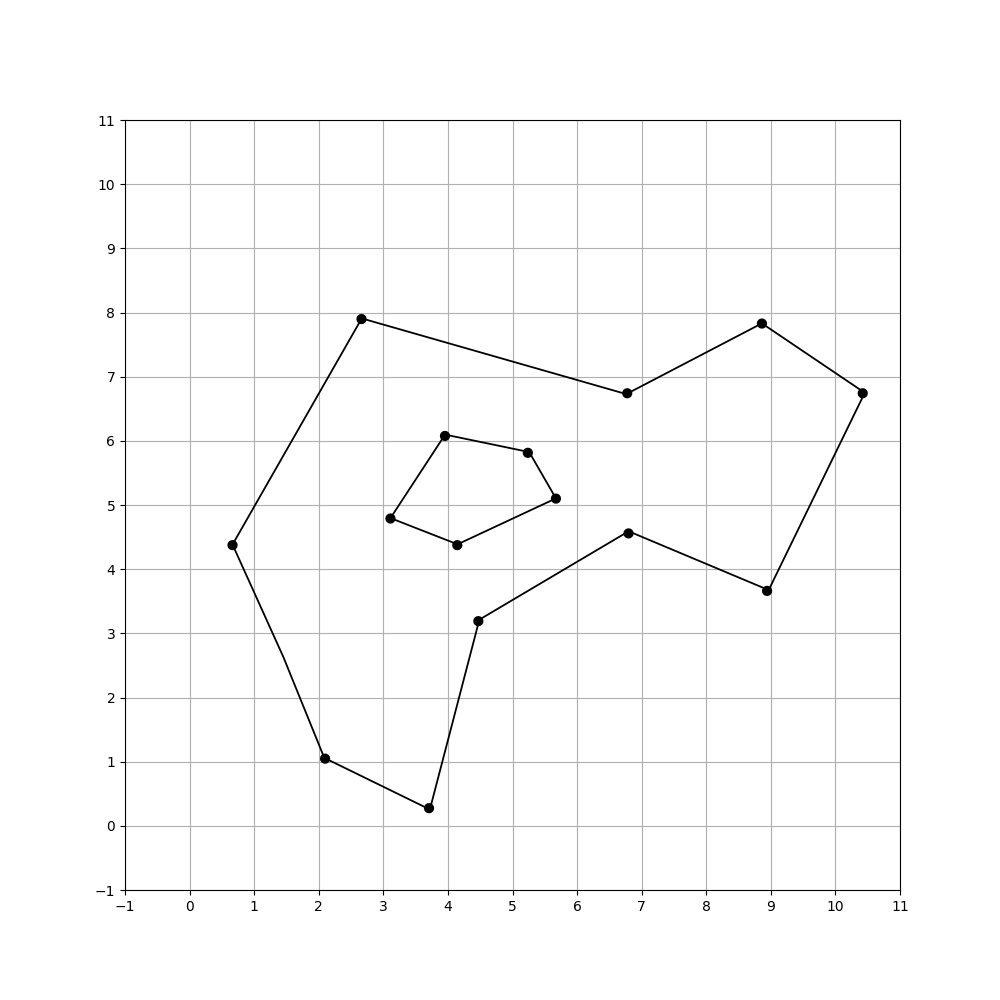
\includegraphics[width=0.50\textwidth]{./Abbildungen/4.png}
    \centering
    \caption{Beispiel eines nicht einfachen, nicht konvexen Polygons}
    \label{viertes beispiel}
\end{figure}
Bevor dieser Algorithmus vorgestellt wird, soll die Beschreibung der dahinterliegenden Grundidee einen Überblick über die Vorgehensweise verschaffen. Danach werden die vorbereitenden Schritte vorgestellt und die Aufteilung des Polygons erläutert. Ein Beispiel dient anschließend zur Veranschaulichung des vorgestellten Algorithmus und zum Schluss des Kapitels wird der Sonderfall geschildert, bei dem Standorte im Inneren des Polygons liegen.

%Die Grundidee des Algorithmus im nicht konvexen Fall
\subsection{Grundidee}\label{grundidee nicht konvex}
In Kapitel~\ref{konvex} wurde bereits erläutert, wie ein einfaches, konvexes Polygon aufgeteilt werden kann. Dieses Vorgehen kann auch bei der Aufteilung nicht konvexer Polygone verwendet werden, muss jedoch in einigen Punkten erweitert werden.\\
Als Voraussetzung wird angenommen, dass ein nicht einfaches, nicht konvexes Polygon $P$ bereits in konvexe Teilpolygone \cpp zerlegt wurde. Im ersten Schritt werden die Teilpolygone mithilfe einer Tiefensuche neu geordnet, um eine feste Bearbeitungsfolge für das weitere Vorgehen zu erhalten. Anschließend werden die Teilpolygone rekursiv aufgeteilt, wie es ähnlich bereits in Kapitel~\ref{konvex} gezeigt wurde. Allerdings können nun Sonderfälle auftreten, die bei der Zerlegung eines einfachen, konvexen Polygons nicht vorkommen können. Einerseits kann \cpi weniger Fläche ausfüllen, als durch \arreq{S(CP_{i})}gefordert ist. In diesem Fall ist \cpi Flächen-unvollständig und muss Flächen von anderen Teilpolygonen übernehmen. Andererseits kann es sein, dass einzelne Teilpolygone keinen Standort enthalten oder weniger Fläche ausfüllen, als durch \arreq{S(CP_{i})}gefordert ist. In diesem Fall ist \cpi Standort-unvollständig und andere Teilpolygone müssen Flächen von \cpi übernehmen.\\
Die Neuordnung wird innerhalb der Prozedur \ord umgesetzt und die Aufteilung inklusive der Sonderfallbehandlung wird durch die beiden Methoden \noncon und \daa umgesetzt, die sich gegenseitig rekursiv aufrufen, bis ein n-Standort Polygon in $n$ 1-Standort Polygone aufgeteilt wurde.

%Beschreibung einer Möglichkeit das Polygon in konvexe Teile zu zerlegen
\subsection{Aufteilung in konvexe Teilpolygone}\label{aufteilung}
Als Voraussetzung für die gleichmäßige Aufteilung eines nicht einfachen, nicht konvexen Polygons wird angenommen, dass das Polygon bereits in konvexe Teilpolygone aufgeteilt wurde. In verschiedenen Werken werden Möglichkeiten einer solchen Aufteilung vorgestellt. Ein Vorgehen wäre zum Beispiel, eine Triangulation eines Polygons zu erzeugen. In diesem Fall würde jedoch eine hohe Anzahl von Teilpolygonen entstehen. Um Teilpolygone zusammenzufassen, könnten nacheinander Kanten der Triangulation entfernt werden, solange das dadurch entstehende Teilpolygon weiterhin konvex ist \cite{Schachter.1978}.
Hieraus wird ersichtlich, dass es verschiedene Möglichkeiten gibt, ein Polygon in konvexe Teilpolygone aufzuteilen. Zum Schluss dieser Arbeit wird besprochen, welche Auswirkungen diese vorbereitenden Schritte auf den Verlauf des vorgestellten Algorithmus haben können.

\begin{figure}[hb]
    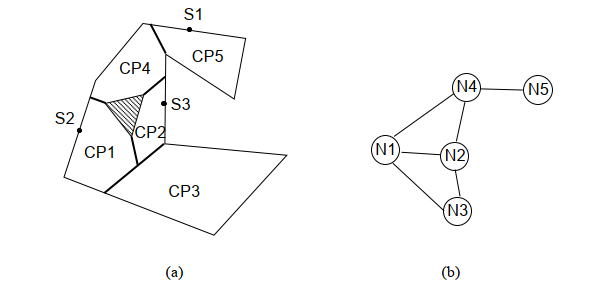
\includegraphics[width=0.70\textwidth]{./Abbildungen/6.png}
    \centering
    \caption{Ein in konvexe Teilpolygone zerlegtes Polygon und dessen Verbindungsgraph. Wenn \ord mit $CP_{1}$ als Eingabe aufgerufen wird, dann werden die verschiedenen Teilpolygone wiefolgt ausgegeben: $CP_{5},CP_{3},CP_{2},CP_{4},CP_{1}$. Das Beispiel ist übernommen aus \cite{Hert.1998}.}
    \label{verbindungsgraph}
\end{figure}
%Beschreibung des Algorithmus um die konvexen Teilpolygone neu zu ordnen
\subsection{Neuordnung der konvexen Teilpolygone}\label{ordnung}

Es kann nun davon ausgegangen werden, dass das Polygon $P$ bereits in konvexe Teilpolygone \cpp zerlegt wurde. Die Teilpolygone können willkürlich geordnet sein und die Indizes treffen keine Aussage über die tatsächliche Anordnung im Polygon $P$. Aus diesem Grund werden die Teilpolygone zuerst neu geordnet, was für den anschließend dargestellten Algorithmus erforderlich ist. Dazu wird ein Verbindungsgraph $G$ gebildet und anhand dessen mittels einer Tiefensuche eine Ordnung erzeugt. Abbildung~\ref{verbindungsgraph} zeigt ein in konvexe Teilpolygone zerlegtes Polygon und dessen Verbindungsgraph.

Jedes Teilpolygon \cpi wird durch einen Knoten $N_{i}$ in $G$ abgebildet. Für jeden Nachbarn $CP_{k} (i \ne k)$ des Teilpolygons \cpi wird eine Kante zum jeweils korrespondierenden Knoten $N_{k}$ eingefügt. \\
Wir definieren einen Knoten $N_{i}$ in $G$ als Blatt, wenn $N_{}$ entweder nur einen Nachbarn hat oder alle Nachbarn von $N_{i}$ als besucht markiert wurden.
Die Prozedur \ord beschreibt nun die Neuordnung der Teilpolygone. \ord wird mit einem beliebigen Knoten $N_{i}$ von $G$ initial aufgerufen. Zuerst wird geprüft, ob $N_{i}$ bereits markiert wurde. Ist dies der Fall, kann der Aufruf zurückkehren. Falls $N_{i}$ noch nicht markiert wurde, wird geprüft, ob $N_{i}$ nach obiger Definition ein Blatt ist. Falls $N_{i}$ kein Blatt ist, dann wird der Knoten markiert und für alle Nachbarn $N_{k}$ von $N_{i}$ rekursiv \ord aufgerufen. Nach dem Rücksprung der Aufrufe aller Nachbarn von \cpi wird \cpi ausgegeben. Falls $N_{i}$ ein Blatt ist, dann wird $N_{i}$ markiert und \cpi ausgegeben. Anschließend wird für alle Nachbarn $N_{k}$ von $N_{i}$ rekursiv \ord aufgerufen.
Die neue Ordnung der \cpi ist nun die Reihenfolge, in der die Teilpolygone ausgegeben wurden.

\begin{lstlisting}[float,caption={Der Algorithmus \ord}, frame=single, label=orderpieces]
// Input: Nj - Node of the connectivity Graph
Function OderPieces(Nj)
    if Nj has not beeing marked then
        if Nj is a leaf node then    
            Mark(Nj)
            Output(CPj)
            for each Nk in Neighbors(Nj)
                OrderPieces(Nk)
        else
            Mark(Nj)
            for each Nk in Neighbors(Nj)
                OrderPieces(Nk)
            Output(CPj)
End OrderPieces(Nj)  
\end{lstlisting}

%Beschreibung des Algorithmus zur Lösung der verankerten Flächenaufteilung im nicht konvexen Fall
\subsection{Aufteilung eines nicht einfachen, nicht konvexen Polygons}\label{aufteilung nicht konvex}
Für die Aufteilung wird jedes Teilpolygon \cpp betrachtet. Konkret wird das Polygon \pred{\mcpi}so aufgeteilt, dass ein Teilstück einem Standort in \cpi (falls vorhanden) zugeordnet wird und der Rest dem Polygon \pred{CP_{k}}mit $k > i$ angehangen wird. Diese Aufteilung wird durch die sich gegenseitig rekursiv aufrufenden Prozeduren \noncon und \daa erreicht. Erstere erzeugt ein Liniensegment, welches \pred{\mcpi}in zwei Teile aufteilt und letztere ordnet die Teile entweder einem Standort zu oder teilt sie erneut auf.

\begin{lstlisting}[float,caption={Der Algorithmus \noncon}, frame=single, label=code nicht konvex]
// Input: Convex polygon CP
Function NonConvexDivide(CP)
    Ls = W(1), Le = W(k)   // k = index of first Site CCW from w1 in W
    PrL, PlL = Cut(CP, L)   // partitioning, returns PrL and PlL
    while Area(PrL) < AreaRequired(S(PrL)) and Le != wm do
       if W(k-1) != S1 and W(k-1) in S then 
          S(CPrL) = S(CPrL) + W(k-1)   // add previous Site to S(CPrL)
       k += 1
       Le = W(k)   // move Le to next point in W
       PrL, PlL = Cut(CP, L)
    if Area(PrL) > AreaRequired(S(CPrL)) then
        if Le == Si then
            k1 = 1
            while Area(PrL) > AreaRequired(S(PrL)) do
                k1 = k1 + 1
                Ls = w(k1)
            L1 = (w(k1), Le)
            T(t1,t2,t3) = (w(k1), w(k1 - 1), Le)
        else
            L1 = (Ls, w(k-1))
            T(t1,t2,t3) = (w(k - 1), w(k1), Ls)
        if Area(PrL1+T) > AreaRequired(S(CPrL)) then
            interpolate point t on (t1,t2) until Area(PrL+T)(*~*)==(*~*)AreaRequired(S(CPrL))
            T(t1,t2,t3) = (t1, t, t3)
            DetachAndAssign(PrL1 + T)
            DetachAndAssign(PlL1 - T - PredPoly(CP,(t1,t))
        else if Area(PrL1+PredPoly(CP,(t1,t2)) < AreaRequired(S(CPrL)) then
            interpolate point t on (t1,t2) until Area(PrL+T)(*~*)==(*~*)AreaRequired(S(CPrL))
            T(t1,t2,t3) = (t1, t, t3)
            DetachAndAssign(PrL1 + T)
            DetachAndAssign(PlL1 - T - PredPoly(CP, (t1,t))
        else
            PS = interiorPoint(t1,t2)   //PS is new Pseudosite
            T(t1,t2,t3) = (t1,PS,t3)
            AreaRequired(PS) = AreaRequired(S(CPrL) - Area(PrL1+T)
            Order(W(PredPoly(CP,(t1,t2))   //such that w1 = PS if Le! = Si and wm = PS if Le == Si
            DetachAndAssign(PredPoly(CP, (t1,t2))
            DetachAndAssign(PrL1 + T)
            DetachAndAssign(PlL1 + T)
    else
        t = InteriorPoint(wm, w1)
        L1 = (t,Si)
        DetachAndAssign(PrL1)
        DetachAndAssign(PlL1)
End NonConvexDivide() 

\end{lstlisting}

Zuerst wird die Prozedur \noncon beschrieben, die die Teilpolygone in zwei Teile aufteilt. Listing~\ref{code nicht konvex} beschreibt diese Prozedur.
Als Eingabe dient ein konvexes Teilpolygon, beschrieben durch die Liste $W(\mcpi)$ (mit $w_{k}, k = 1,…,m$) mit allen Polygonpunkten inklusive Steiner-Punkten und die Liste $S(\mcpi)$ mit den Standorten des Teilpolygons inklusive der jeweils benötigten Fläche.
Anders als bei \con aus Kapitel~\ref{konvex} ist für die Bearbeitung relevant, welche Punkte $w_{1}$ und $w_{m}$ in $W(\mcpi)$ sind. Die Kante, die durch die Polygonpunkte $(w_{m}, w_{1})$ erzeugt wird, sei nun die Kante zu $NextNeighbor(\mcpi)$. Hat \cpi keinen nächsten Nachbarn, muss $w_{m}$ gleich einem Standort sein. Weiterhin gilt, dass $W(\mcpi)$ wieder gegen den Uhrzeigesinn geordnet ist.\\

Wie es auch schon bei \con der Fall war, lässt die Prozedur erneut ein Liniensegment \l gegen den Uhrzeigersinn durch das Polygon \cpi wandern, wobei \ls als Drehpunkt dient. \l wird durch $(L_{s}, L_{e}) = (w_{1}, S_{i})$ initialisiert, wobei $S_{i}$ der erste Standort aus $S(\mcpi)$ ist.\\
Nun können zwei Fälle eintreten, in denen die Schleife stoppt:

\begin{itemize}
\item Die Fläche rechts der Linie \l ist größer oder gleich der benötigten Fläche der Standorte, die sich in diesem Gebiet befinden. Es gilt:
$\mar{\mprl}\ge\marreq{S(\mcprl)}$
\item Das Ende des Polygons wird erreicht, also \Le $= w_{m}$.
\end{itemize}

Durch die Bearbeitung von vorherigen Teilpolygonen kann es sein, dass nicht zugewiesene Teile dieser Polygone in die Aufteilung von \cpi miteinbezogen werden müssen. Außerdem kann nun der Fall eintreten, dass die Fläche des Teilpolygons kleiner ist als $AreaRequired(S(\mcpi))$. Aus diesem Grund müssen die oberen beiden Fälle noch feingranularer aufgeteilt werden.\\

\textbf{Fall 1:} Wie auch in der Prozedur \con wird ein Ende der Linie $L$ entlang des Polygons bewegt, um die Fläche \ar{\mprl}zu verkleinern. Hierbei unterscheiden wir zwei Fälle. Falls $L_{e} = S_{i}$ für einen beliebigen Wert für $i$ gilt, dann wird der Startpunkt \ls gegen den Uhrzeigersinn bewegt, ansonsten wird der Endpunkt \Le im Uhrzeigersinn bewegt.

Nun seien \leins und \lzwei zwei Liniensegmente, die einen gemeinsamen, festen Endpunkt haben. Dieser gemeinsame Endpunkt ist für beide Linien entweder \ls oder \Le und damit das Gegenstück zum oben bestimmten Punkt, welcher entlang des Polygons bewegt wird. Die Linien sind so positioniert, dass $\mar{P^{r}_{L_{1}}} < \marreq{S(CP^{r}_{L_{1}})}$ und $\mar{P^{r}_{L_{2}}} > \marreq{S(CP^{r}_{L_{2}})}$ gilt. Die Linie \lzwei wird demnach durch $(w_{1}, w_{k})$ und die Linie \leins durch $(w_{1}, w_{k-1})$ beschrieben.
Dadurch entsteht ein Dreieck $T = (t_{1}, t_{2}, t_{3})$, das die Differenz von \cprleins und \cprlzwei bildet. Außerdem sei $(t_{1}, t_{2})$ das Liniensegment von $\mcpi$, das $L_{1}$ und $L_{2}$ verbindet. Der gemeinsame Endpunkt von \leins und \lzwei ist demnach $t_{3}$.

Nun muss \cprleins mit einer Teilfäche des Dreiecks $T$ und gegebenenfalls mit Teilflächen der Reste der Vorgängerpolygone vereinigt werden, damit die Flächenanforderungen der Standorte in \cprleins erfüllt werden. Dabei entstehen 3 Fälle:

\begin{itemize}
\item $\mar{\mprleins + T} > \marreq{S(\mcprl)}$ \\
Die Flächenanforderung der Standorte kann durch die Fläche rechts von \leins und $T$ vollständig gedeckt werden. Insbesondere wird kein Flächenanteil von \predl{CP}{t_{1},t{2}}benötigt. 
\item $\mar{\mprleins +T} \le \marreq{S(\mcprl)}$ und \\ $\mar{\mprleins+PredPoly(CP,(t_{1},t_{2}))}<\marreq{S(\mcprl)}$ \hfill ($\ast$) \\
Die Flächen von \prleins und $T$ reichen zusammen nicht $(<)$ oder exakt $(=)$ aus, um die Flächenanforderung der Standorte von \cprl zu erfüllen (1. Bedingung). Weiterhin liegt der Fall vor, dass die Fläche von \prleins in Kombination mit dem Vorgängerpolygon \linebreak \predl{CP}{t_{1},t_{2}} kleiner als die geforderte Fläche ist (2. Bedingung).
\item $\mar{\mprleins +T} \le \marreq{S(\mcprl)}$ und \\ $\mar{\mprleins+PredPoly(CP,(t_{1},t_{2}))}\ge\marreq{S(\mcprl)}$ \\
Bedingung 1 ist analog zu Fall 1.2. Weiterhin liegt nun jedoch der Fall vor, dass die Fläche von \prleins in Kombination mit dem Vorgängerpolygon \predl{CP}{t_{1},t_{2}}zur Erfüllung der Anforderung genügt (2. Bedingung).
\end{itemize}

Die je nach Fall entstehenden Polygone werden anschließend an die Prozedur \daa übergeben und dort entweder Standorten zugewiesen oder durch einen rekursiven Aufruf von \noncon erneut aufgeteilt.\\

\textbf{Fall 1.1:} Die Flächenanforderung von $S(\mcprl)$ kann durch das Polygon \prleins zusammen mit dem Dreieck $T$ erfüllt werden. In diesem Fall reicht es aus, mittels linearer Interpolation einen Punkt $t$ zwischen $t_{1}$ und $t_{2}$ zu finden, sodass für das Dreieck $T' = (t_{1}, t, t_{3})$ gilt:
\begin{align*}\mar{\mprleins+T'-PredPoly(CP,(t_{1},t))}=\marreq{S(\mcprl)} \end{align*}
Durch diese Aufteilung entstehen die beiden Polygone $(\mprleins + T' - PredPoly(CP,(t_{1},t))$ und \hbox{$(\mprleins -T')$}, die der Prozedur \daa übergeben werden.\\

\textbf{Fall 1.2:} Damit die Flächenanforderung erfüllt werden kann, wird zunächst das Vorgängerpolygon \predl{CP}{t_{1},t_{2}}hinzugenommen und dieses um die Fläche \prleins und einen Teil des Dreiecks T erweitert. Erneut wird durch lineare Interpolation der Punkt t gefunden und wie oben das Dreieck $T'$ gebildet, sodass die Flächenanforderung erfüllt ist. Das Dreieck $T'$ kann durch die strikte Ungleichung $(\ast)$ nicht kollabieren. Somit entstehen die beiden Polygone $(\mprleins + T')$ und $(\mprleins - T' - PredPoly(CP,(t_{1},t))$, die der Prozedur \daa übergeben werden.\\

\textbf{Fall 1.3:} Die Fläche der Vorgängerpolygone ist größer als die Flächenanforderung der Standorte. In diesem Fall muss die Fläche der Vorgängerpolygone wiederrum aufgeteilt werden. Ein Teil wird zur Erfüllung der Flächenanforderung genutzt und $S(\mcprleins)$ zugeordnet. Der übrige Teil wird im Weiteren durch einen sogenannten Pseudostandort $PS$ abgebildet. $PS$ wird auf der Kante zwischen $t_{1}$ und $t_{2}$ willkürlich hinzugefügt, sodass das Dreieck $T' = (t_{1}, PS, t_{3})$ entsteht. Es gilt:
\begin{align*}\marreq{PS}=\marreq{S(\mcprl) - \mar{\mprleins + T'}} \end{align*}
$PS$ bekommt also die fehlende Flächenanforderung zugewiesen. Dadurch kann \linebreak \predl{CP}{t_{1},PS} ebenfalls durch \noncon aufgeteilt und ein Teilpolygon $PS$ zugewiesen werden. Das zugewiesene Teilpolygon kann dann dem Polygon $(\mprleins + T')$ hinzugefügt werden. Dieses Polygon und das Polygon $(\mplleins -T')$ werden dann an \daa übergeben. \\

Weiterhin muss der Fall betrachtet werden, bei dem das Liniensegment $L$ das Polygon einmal komplett durchlaufen hat.\\
\textbf{Fall 2:} Dieser Fall tritt ein, wenn ein Teilpolygon und die Reste der Vorgängerpolygone weniger Fläche enthalten, als die Standorte beanspruchen. In diesem Fall ist \cpi Flächen-unvollständig und es muss für mindestens einen Standort aus $S(\mcprl)$ ein Pseudostandort erzeugt werden. Dazu wird ein Punkt $t$ auf der Kante $(w_{m}, w_{1})$ erzeugt, also der Kante zu \next{\mcpi}. Nun sei $L = (t, S_{i})$, wobei \si der erste Standort in $S(\mcpi)$ gegen den Uhrzeigersinn von $w_{1}$ aus ist. Nun wird $W(\mprl)$ so geordnet, dass $t = w_{1}$ gilt. Anschließend werden \prl und \pll an \daa übergeben. Hierbei entsteht entweder auf dem Liniensegment $(w_{1}, w_{2})$ ein Pseudostandort oder ein Teil von \prl wird dem Standort \si zugeordnet. Wenn ein Pseudostandort entsteht, dann wird diesem die Flächenanforderung von \si abzüglich der Fläche von \prl zugeordnet und das Polygon \prl von \cpi entfernt. Mit den restlichen Standorten von \cpi wird dasselbe Verfahren angewandt.\\
Die Pseudostandorte werden nun bei der Aufteilung von \next{\mcpi}behandelt. Wenn den Pseudostandorten hierbei ein Polygon zugeteilt wird, dann wird dieses Polygon auf die korrespondierenden Standorte übertragen.\\
Zusammenfassend wird durch den Algorithmus von \noncon ein $q$-Standort-Polygon entweder in ein $q_{1}$-Standort-Polygon und ein $q_{2}$-Standort-Polygon mit $q_{1}, q_{2} > 0$ und $q_{1} + q_{2} = q$ aufgeteilt oder es wird ein $1$-Standort Polygon abgetrennt und es bleibt ein $q'$-Standort Polygon mit $q' = q - 1$ übrig.

%Beschreibung des Algorithmus DetachAndAssign
\subsection{Der Algorithmus DetachAndAssign}\label{detach}

\begin{lstlisting}[float,caption={Der Algorithmus \daa}, frame=single, label=code detach]
// Input: Poly(CP) - Polygon rooted at convex piece CP
Function DetachAndAssign(Poly(CP))
    if Length(S(CP)) == 0 then return 
    if PredPoly(CP) is AreaComplete then
        if S(CP) == {Si} then   //for some i
            Assign PredPoly(CP) to Si
            Detach PredPoly(CP) from Poly(CP)
        else
            Detach PredPoly(CP) from Poly(CP)
            Order(W(CP))   //such that wm = Si for some i
            NonConvexeDivide(CP)
    else if PredPoly(CP) is areaIncomplete then
        if S(CP) == {Si} then	//for some i
             Assign PredPoly(CP) to Si
             Detach PredPoly(CP) from Poly(CP)
             PS = interiorPoint(w(j),w(k))   //with (w(j),w(k)) is edge to NextNeighbor(CP)
        else
            Order(W(CP))   //such that edge (w(m),w(1)) is edge to NextNeighbor(CP)
            NonConvexeDivide(CP)
    else
        Order(W(CP))   //such that edge (w(m),w(1)) is edge to NextNeighbor(CP)
        NonConvexeDivide(CP)
End DetachAndAssign()

\end{lstlisting}

Die Prozedur \daa teilt ein Polygon einem Standort zu oder teilt ein Teilpolygon erneut mittels \noncon auf. \daa ist durch Listing~\ref{code detach} beschrieben.

Beim Aufruf von \emph{DetachAndAssign(Poly(CP))} können 3 Fälle auftreten. Das Polygon
\begin{itemize}
\item \pred{CP} ist Flächen-vollständig
\item \pred{CP} ist Flächen-unvollständig
\item \pred{CP} ist Standort-unvollständig
\end{itemize}
Im ersten Fall kann es sein, dass \pred{CP} nur einen Standort besitzt. Dann kann\linebreak \pred{CP} vom Polygon $Poly(CP)$ getrennt (\emph{Detach}) und komplett diesem Standort zugeteilt (\emph{Assign}) werden.
Falls \pred{CP}mehrere Standorte enthält, wird \pred{CP}von $Poly(CP)$ getrennt und rekursiv mittels \noncon aufgeteilt. \\
Im zweiten Fall treten die gleichen zwei Unterfälle auf. Falls \pred{CP}nur einen Standort \si hat, kann \pred{CP}von $Poly(CP)$ getrennt und dem Standort zugeteilt werden. Da \pred{CP}Flächen-unvollständig ist, muss nun ein Pseudostandort auf der Kante zu \next{CP}erzeugt werden, der die restliche Flächenanforderung von \si enthält. Flächen, die im weiteren Verlauf dem Pseudostandort zugeteilt werden, werden so mittelbar dem Standort \si zugeteilt.
Falls \pred{CP}mehrere Standorte hat, dann wird \pred{CP}zunächst neu geordnet, sodass $(w_{m}, w_{1})$ die Kante zu \next{CP}ist. Anschließend erfolgt wiederum ein rekursiver Aufruf von \mbox{\textit{NonConvexDivide}}, da nicht bekannt ist, durch welchen Standort die Flächen-Unvollständigkeit resultiert.\\
Im dritten Fall hat \pred{CP}mehr Fläche, als die Standorte von $CP$ benötigen. In diesem Fall wird \pred{CP}ebenfalls neu geordnet, sodass $(w_{m}, w_{1})$ die Kante zu \next{CP} ist. Mit diesem Polygon erfolgt ein Aufruf von \mbox{\textit{NonConvexDivide}}.

Abbildung~\ref{beispiel nicht konvex} zeigt ein Beispiel einer Zerlegung eines nicht konvexen Polygons.

%Beschreibung des Sonderfalls, wenn Standorte innerhalb des Polygons liegen
\subsection{Behandlung innen liegender Standorte}\label{innere Standorte}
Für innen liegende Standorte muss die in Kapitel~\ref{aufteilung} beschriebene Zerlegung in konvexe Teilpolygone so erfolgen, dass jeder Standort anschließend auf einer Kante liegt. Ist dies nicht direkt möglich, können für die Standorte auch weitere Kanten eingefügt werden und die Aufteilung in konvexe Teilpolygone wird etwas detaillierter. Die neuen Kanten laufen durch die innenliegenden Standorte. Für den korrekten Ablauf des Algorithmus spielt diese Art der Zerlegung keine Rolle.


%Komplexitätsanalyse der Vorgestellten Algorithmen
\section{Komplexitätsanalyse}\label{komplex}
%Konvexer Fall
\subsection{Konvexes Polygon}
Der Algorithmus \con benötigt lineare Zeit bezogen auf die Anzahl der Elemente der Liste $W(P)$, um einen einzelnen Schnitt durchzuführen. Der dabei erforderliche Aufbau der Polygone \prl beziehungsweise \pll sowie die Ermittlung der Fläche ist in konstanter Zeit möglich. Das Finden der Punkte, bei denen $\mar{\mprl} = \marreq{S(\mprl)}$ gilt, kann ebenso in konstanter Zeit erfolgen. Der Algorithmus \con benötigt daher $O(n+v)$ Zeit ($n$ = Anzahl der Standorte, $v$ = Anzahl an Polygonpunkten).\\
Im ungünstigsten Fall trennt \con von einem konvexen Polygon mit $q$ Standorten nur ein Dreieck ($v$ = 3, $n$ = 1) ab. Neben dem Dreieck verbleibt dann ein konvexes Polygon mit $q-1$ Standorten und $v+1$ Polygonpunkten. Für dieses Polygon gilt wiederum selbes. Um eine gesamte Flächenzerlegung eines konvexen Polygons zu berechnen, wird $O((n-1)(n+v))$ Zeit benötigt. 
Hierbei sei angemerkt, dass dieser Algorithmus stets terminiert, da die Anzahl an Standorten konstant ist und die Anzahl der Teilpolygone je Schnitt um 1 erhöht wird. Nach $n-1$ Schnitten entspricht die Anzahl der Teilpolygone der Anzahl der Standorte.
%Nicht konvexer Fall
\subsection{Nicht konvexes Polygon}
Der Algorithmus \ord besucht jeden Knoten im Nachbarschaftsgraphen maximal zwei Mal, sodass die Ordnung in linearer Zeit $O(p)$ bezogen auf die Anzahl $p$ der konvexen Teile erfolgen kann.
Der Algorithmus \noncon benötigt $O(pn^{2} + nv)$ Zeit, um alle $p$ konvexen Teile unter den $n$ Standorten aufzuteilen. Im ungünstigsten Fall wird jedes der $p$ konvexen Teile in $n$ Polygone zerlegt, wobei jedes der Polygone einen Teil eines Standorts abbildet.\\
Der Algorithmus \daa wird getrennt für den Teil \emph{Detach} beziehungsweise \emph{Assign} betrachtet.\\
Um ein Polygon nach einem Schnitt zu lösen (\emph{Detach}), müssen alle Zeiger auf Nachbarpolygone aktualisiert werden. Dieser Vorgang ist in Zeit $O(v_{j})$ für ein konvexes Polygon mit $v_{j}$ Polygonpunkten möglich. Der ungünstigste Fall beziehungsweise die maximale Anzahl an zu aktualisierenden Zeigern besteht dann, wenn je Zerlegung ein Dreieck $(v=3)$ und ein Polygon mit $v_{j}+1$ Polygonpunkten abgetrennt werden. Für alle Teilpolygone ergibt sich dann eine maximale Zeit von $O(v + pn^{2})$.\\
Der Algorithmus \emph{Assign} übernimmt die Zuweisung von Flächen zu Standorten, wobei eine Fläche aus einem Set von konvexen Teilen besteht. Die Vereinigung der konvexen Teile zu einem Polygon benötigt lineare Zeit bezogen auf die Anzahl der Polygonpunkte aller Teile, also maximal $O(pn + v)$. Die Vereinigung aller $n$-Standort-Polygone benötigt daher $O(pn^{2}+ vn)$ Zeit. 
Zusammenfassend ergibt sich aus den Laufzeiten für \mbox{\textit{OrderPieces}}, \noncon und \daa eine Gesamtlaufzeit von $O(pn^{2} + vn)$.

%Schluss und Ausblick
\section{Schluss und Ausblick}\label{schluss}
In dieser Arbeit wurde das \emph{Problem der verankerten Flächenaufteilung} vorgestellt und anhand von Beispielen für konvexe und nicht konvexe Polygone erläutert.
Sowohl der beschriebene Algorithmus für ein konvexes Polygon, als auch die verallgemeinerte Version für ein nicht konvexes, nicht einfaches Polygon liefern für ein gegebenes Problem eine Lösungen.

Weitere Untersuchungsmöglichkeiten für die Anpassung und Optimierung des Algorithmus liegen beispielsweise für den konvexen Fall in der Reihenfolge der Punkte des Eingangspolygons beziehungsweise für den nicht konvexen Fall in derArt der Aufteilung des Polygons in konvexe Teilpolygone $CP_{i}$. Weitergehende Forschung könnte den Einfluss dieser Parameter auf die Form der entstehenden Polygone untersuchen. Unter anderem könnte es für die Roboterplanung von Vorteil sein, wenn die resultierenden Flächen möglichst einfach und kompakt (im Sinne des kleinesten umschließenden Durchmessers) sind, da Roboter auf solchen Flächen typischerweise effizienter arbeiten.


\section{Abkürzungs- und Begriffsverzeichnis}\label{begriffe}
\begin{tabular}[t]{ | p{ 0.3\textwidth} | p{ 0.65\textwidth } |  }
\hline
 \rowcolor{lightgray} Abkürzung/Begriff & Bedeutung\\
\hline
c & Geforderter Flächenanteil des Standorts $S$ am zugehörigen Polygon $P$ mit $0 < c < 1$ \\
\hline
$CP$ & Ein konvexes Polygon \\
\hline
FE & Flächeneinheiten \\
\hline
$L$ & Liniensegment, orientiert von \ls nach \Le \\
\hline
\ls & Startpunkt des Liniensegments L\\
\hline
\Le & Endpunkt des Liniensegments L\\
\hline
$P$ & Polygon \\
\hline
$\mcprl$ & Teilpolygon rechts des Liniensegments L \\
\hline
$\mcpll$ & Teilpolygon rechts des Liniensegments L \\
\hline
$S$ & Standort \\
\hline
Steiner-Punkt & Polygonpunkt, welcher nicht Teil des Eingangspolygons ist und während der Lösung eines geometrischen Problems hinzugefügt wird \\
\hline
q-Standort-Polygon & Polygon mit insgesamt q Standorten \\
\hline
$V(P)$ & Liste der Polygonpunkte von $P$, inklusive aller Steiner-Punkte, gegen den Uhrzeigersinn geordnet \\
\hline
$S(P)$ & Liste der zu $P$ zugeordneten Standorte $S_{i}$, in der Reihenfolge ihres Vorkommens gegen den Uhrzeigersinn geordnet, beginnend mit $v_{1}$\\
\hline
$W(P)$ & Liste der Polygonpunkte und Standorte von $P$, d.h. $S(P) + V(P)$, wobei $w_{1} \in V(P)$ bzw. $w_{1} \notin S(P)$ gilt\\
\hline
\ar{P} & Flächeninhalt des Polygons P \\
\hline
\arreq{S(P)} & Benötigte Fläche der Standorte im Polygon P, berechnet mit $c*\mar{P}$ \\
\hline
Flächen-vollständig & Wenn für ein Polygon $P$ gilt: $\mar{P} = \marreq{P}$ \\
\hline
Flächen-unvollständig & Wenn für ein Polygon $P$ gilt: $\mar{P} < \marreq{P}$ \\
\hline
Standort-unvollständig & Wenn für ein Polygon $P$ gilt: $\mar{P} > \marreq{P}$ \\
\hline
Nachbar & Zwei Teilpolygone, die eine gemeinsame Kante haben, werden als Nachbarn bezeichnet \\
\hline
Vorgänger von \cpi & Alle Teilpolygone $CP_{k}$, die eine kleinere Ordnung als \cpi haben und es einen Weg im Verbindungsgraph von \cpi nach $CP_{k}$ gibt \\
\hline
Nachfolger & Alle Teilpolygone $CP_{k}$, die eine größere Ordnung als \cpi haben und es einen Weg im Verbindungsgraph von \cpi nach $CP_{k}$ gibt \\
\hline
\next{\mcpi} & Ein Nachbarpolygon des Teilpolygons $\mcpi$, das ein Nachfolger von \cpi ist und die kleinste Ordnung hat \\
\hline

\end{tabular}

\begin{tabular}[t]{ | p{ 0.3\textwidth} | p{ 0.65\textwidth } |  }
\hline
 \rowcolor{lightgray} Abkürzung/Begriff & Bedeutung\\
\hline
\pred{\mcpi} & \cpi und alle von \cpi aus erreichbaren Vorgänger, ohne dabei einen Nachfolger zu schneiden \\
\hline
\predl{\mcpi}{e} & \cpi und alle von \cpi aus über die Kante $e$ erreichbaren Vorgänger, ohne dabei einen Nachfolger zu schneiden \\
\hline
$Poly(\mcpi)$ & \cpi und alle von \cpi aus erreichbaren Teilpolygone \\
\hline
\prl & \cprl und \predl{\mcpi}{e}, für alle Kanten, die rechts der Linie $L$ verlaufen oder einen Endpunkt auf $L$ haben \\
\hline
\pll & $\mcpll$ und \predl{\mcpi}{e}, für alle Kanten, die links der Linie $L$ verlaufen oder einen Endpunkt auf $L$ haben \\
\hline
\end{tabular}


\begin{figure}[hb]
\begin{center}
    \subfloat[]{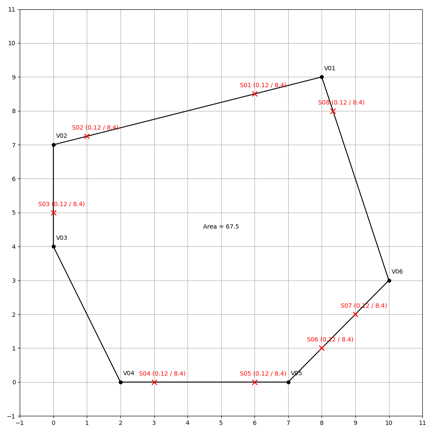
\includegraphics[width=0.30\textwidth]{./Abbildungen/3a.png}}
    \subfloat[]{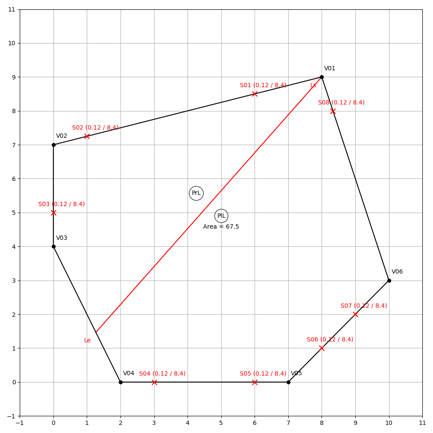
\includegraphics[width=0.30\textwidth]{./Abbildungen/3b.png}}
    \subfloat[]{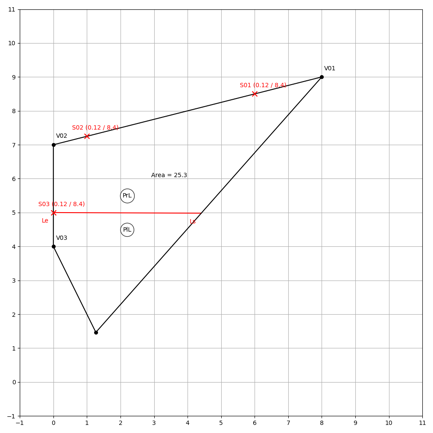
\includegraphics[width=0.30\textwidth]{./Abbildungen/3c.png}}
    \qquad
    \subfloat[]{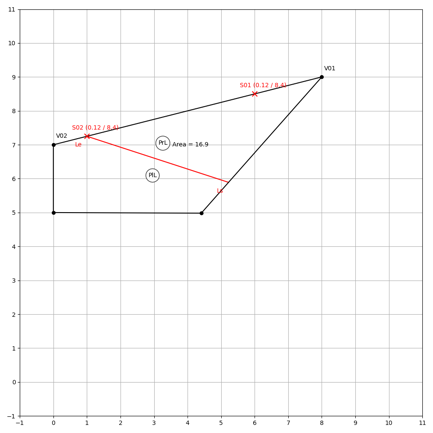
\includegraphics[width=0.30\textwidth]{./Abbildungen/3d.png}}
    \subfloat[]{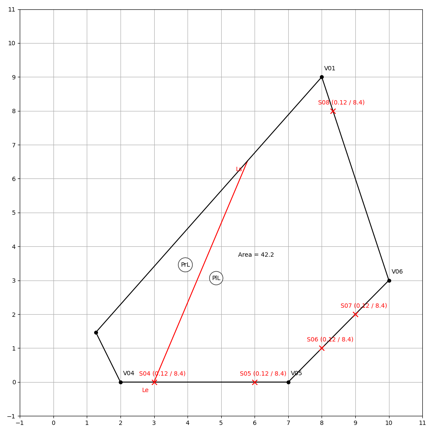
\includegraphics[width=0.30\textwidth]{./Abbildungen/3e.png}}
    \subfloat[]{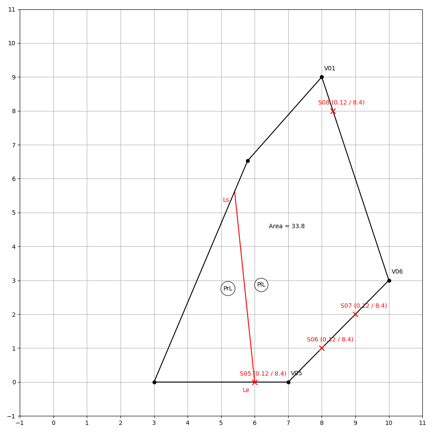
\includegraphics[width=0.30\textwidth]{./Abbildungen/3f.png}}
    \qquad
    \subfloat[]{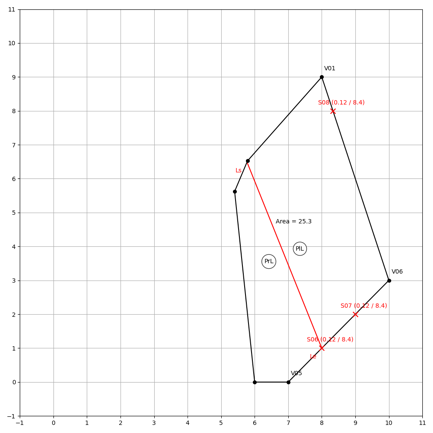
\includegraphics[width=0.30\textwidth]{./Abbildungen/3g.png}}
    \subfloat[]{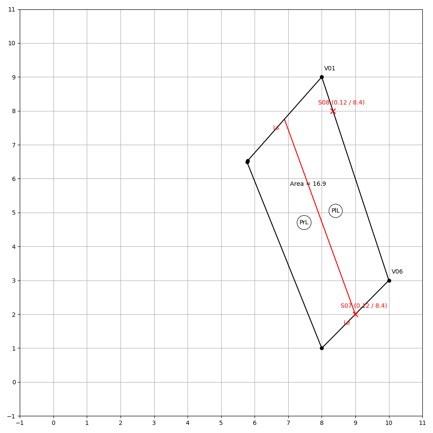
\includegraphics[width=0.30\textwidth]{./Abbildungen/3h.png}}
    \subfloat[]{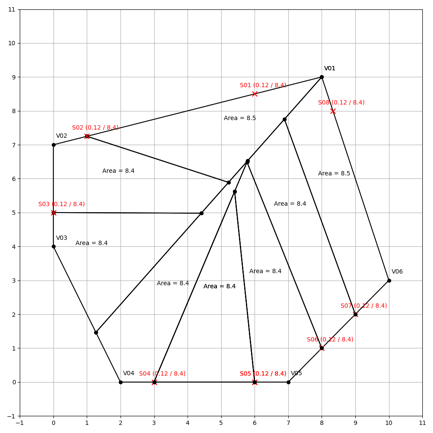
\includegraphics[width=0.30\textwidth]{./Abbildungen/3i.png}}
\end{center}
\caption{\small Beispiel einer gleichmäßigen Aufteilung eines konvexen Polygons mit acht Standorten und einem jeweils benötigen Flächenanteil von $12,5\%$. (a) zeigt hierbei das Ausgangspolygon $CP$ mit dem ersten Polygonpunkt bei Koordinate $(8, 9)$ und den im Gegenuhrzeigersinn geordneten Standorten $S01$ bis $S08$. In (b) liegt zunächst Fall 2.1 vor, bei welchem \Le bis $V04$ bewegt wird, sodass $\mar{\mprl} > \marreq{S(\mprl)}$ gilt. $S(\mprl)$ enthält in diesem Zustand die Standorte $S01$ bis $S03$. Für \Le wird anschließend eine Interpolation zwischen $V04$ und $V03$ durchgeführt, sodass $\mar{\mprl} = \marreq{S(\mprl)}$ gilt und es wird ein Schnitt durchgeführt. Für das rechts der Schnittlinie entstandene Polygon wird in (c) erneut \con aufgerufen. Hierbei tritt Fall 2.2 ein. \Le erreicht bei der Verschiebung $S03$, welcher letzter Standort in \s ist. \ls wird anschließend im Uhrzeigersinn inkrementell bewegt, bis $\mar{\mprl} = \marreq{S(\mprl)}$ gilt. Erneut muss das rechts der Schnittlinie entstandene Polygon aufgeteilt werden, siehe (d). \Le wandert wieder bis zum letzten Standort in $S()$, sodass erneut Fall 2.2 vorliegt. Dass \ar{\mprl} bei $L_{e} = S_{n}$ eine Fläche von 0 aufweist, stellt für den Algorithmus kein Problem dar. In (e) wird nun das in (b) links der Schnittlinie entstandene Polygon weiter aufgeteilt. Es liegt Fall 1 vor, da nach der Initialisierung mit $L_{e} = S_{1}$ bereits $\mar{\mprl} > \marreq{S(\mprl)}$ gilt. \ls wird anschließend gegen den Uhrzeigersinn verschoben, bis $\mar{\mprl} = \marreq{S(\mprl)}$ vorliegt. In den nächsten Schritten (f)-(h) gilt analog Fall 1. Speziell in (f) soll darauf hingewiesen werden, dass das inkrementelle Verschieben des Punktes \ls auch über eine Polygonecke hinaus möglich sein muss. (i) zeigt die resultierende Flächenaufteilung aus den Schritten (b) - (h) mit Teilflächen zu je $12,5\%$.}
\label{beispiel konvex}
\end{figure}


\begin{figure}[hb]
\begin{center}
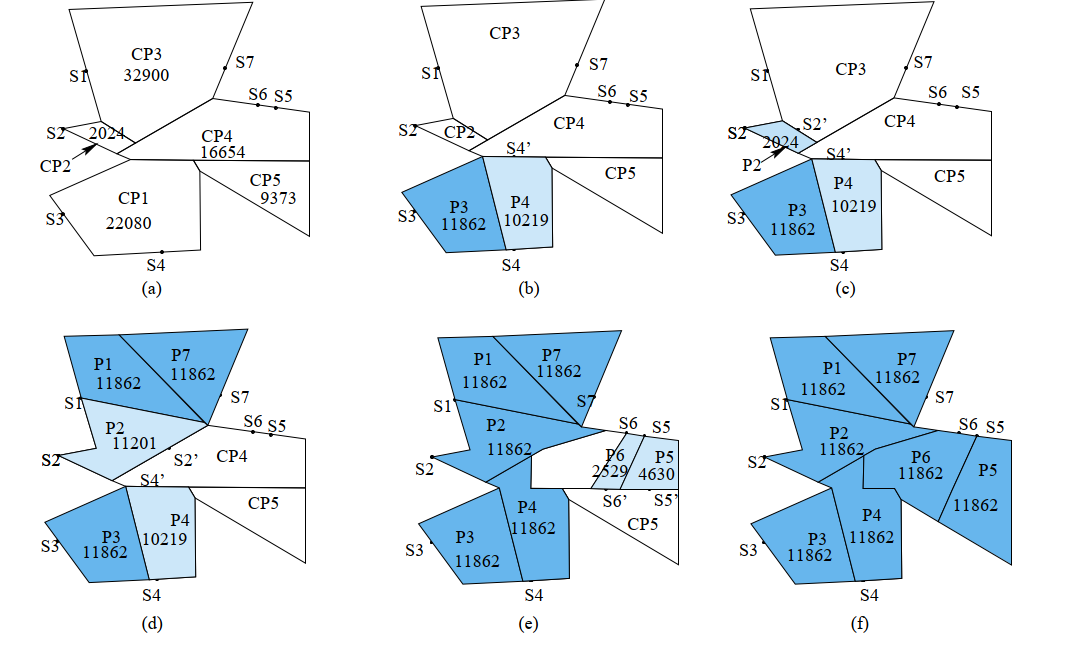
\includegraphics[width=1\textwidth]{./Abbildungen/5.png}   
\end{center}
\caption{\small Beispiel einer Aufteilung eines nicht konvexen Polygons, entnommen aus \cite{Hert.1998} Abbildung 17\\
Gezeigt sind hier die verschiedenen Stadien der gleichmäßigen Aufteilung eines nicht konvexen Polygons mit 12 Ecken und sieben Standorten. (a) zeigt die initiale Aufteilung des Polygons in 5 konvexe Teilpolygone $CP1, …,CP5$. In (b) – (f) werden die Teilpolygone, die bereits einem Standort zugeteilt sind, dunkelblau markiert. Die Teilpolygone, die bereits einem Standort zugeteilt, aber noch Flächen-unvollständig sind, werden hellblau markiert.\\
In (b) wird das Teilpolygon $CP1$ bearbeitet und dabei in zwei Teilpolygone aufgeteilt. $P3$ wird dem Standort $S3$ zugeordnet und $P4$ dem Standort $S4$. $P4$ erfüllt die Flächenanforderung von $S4$ nicht vollständig, weshalb ein Pseudostandort $S'4$ an der Kante zu \next{CP1}erzeugt wird. Dieser Pseudostandort wird zu einem späteren Zeitpunkt bearbeitet.\\
 (c) zeigt den Zustand nach der Bearbeitung von Teilpolygon $CP2$. Hier tritt erneut der Fall auf, dass die Fläche, die dem Standort $S2$ zugeteilt wird, zu klein ist. Aus diesem Grund wird der Pseudostandort $S'2$ an der Kante zu \next{CP2}erzeugt.\\
In (d) wird der Zustand nach der Bearbeitung von Teilpolygon $CP3$ gezeigt. Dort wird das Teilpolygon $P7$ dem Standort $S7$ zugeteilt und das Teilpolygon $P1$ dem Standort $S1$. Der Rest von $CP3$ wird mit $P2$ vereint und daher ebenfalls $S2$ zugewiesen. Da die Fläche von $P2$ weiterhin nicht groß genug ist, um der Flächenanforderung von $S2$ zu genügen, wird ein neuer Pseudostandort $S'2$ an der Kante zu \next{CP3}erzeugt.\\
 (e) zeigt den Zustand nach der Bearbeitung von $CP4$. Dort hat das Liniensegment das Ende von $CP4$ erreicht, ohne dass zuvor die Flächenanforderung der Standorte erfüllt werden konnte. Aus diesem Grund wird $P5$ und der Pseudostandort $S'5$ erzeugt und diese $S5$ zugeordnet. Anschließend wird derselbe Schritt für $S6$ wiederholt. Nach Abziehen der Flächen $P5$ und $P6$ von $CP4$ werden Teile von $CP4$ den Pseudostandorten $S'2$ und $S4$ zugeordnet und mit den Teilpolygonen $P2$ und $P4$ vereint.\\
Im letzten Schritt (f) wird $CP5$ und der verbliebene Teil von $CP4$ den Pseudostandorten $S5$ und $S6$ zugeordnet. Die Abbildung zeigt das in gleichmäßige Teilpolygone $P1,…,P7$ zerlegte Polygon.}
\label{beispiel nicht konvex}
\end{figure}

\bibliographystyle{abbrv}
\bibliography{literatur} % Daten aus der Datei literatur.bib verwenden.



\end{document}

